\documentclass[11pt]{article}
\usepackage{fullpage,amsthm,amsfonts,amssymb,epsfig,amsmath,times,amsthm}
\usepackage{tabu}
\usepackage{pgfplots}
\usepackage{tikz}
\usetikzlibrary{arrows}

\newtheorem{theorem}{Theorem}
\newtheorem{claim}[theorem]{Claim}
\newcommand\tab{\setlength\parindent{24pt}}

\begin{document}

	\begin{center}
		{\bf\Large CMPS 102 --- Fall 2018 --  Homework 4}\\
		Alyssa Melton\\
		I have read and agree to the collaboration policy. \\
		Collaborators: none\\
	\end{center}

	%------------------------------------------------------------------------------
	%------------------------------------------------------------------------------

	\section*{Solution to Problem 1}
		Charlie only likes two coffee shops, Valve and Ruru. For each minute at either coffee shop, we know precisely how productive Charlie will be, aka, we know how much work he will get done. This is given in the following sets:\\
		\\
		$V=\{v_1, v_2, . . . , v_i. . . , v_n\}$\\
		\\
		$R=\{r_1, r_2, . . . , r_i, . . . , r_n\}$\\
		\\
		While thinking of ways I can think of this problem, I considered creating a graph with weighted edges that represent the amount of work that Charlie can get done in between two minute marks.\\
		\\
		In the graph below, I am considering time being at the earliest at the top, and the latest at the bottom.\\
		\\
		The minutes that Charlie can either spend at Valve or Ruru are vertices, namely $V_1$ to $V_n$, and $R_1$ to $R_n$ respectively.\\
		\\
		We create edges connecting each consecutive minute at the same coffee shop, making a direct path though $V_1$ to $V_n$, and the same with $R_1$ to $R_n$. For an edge $(C_i, C_{i+1})$, where $C$ is the coffee shop (either $V$ or $R$) and $i$ is the minute, $(C_i, C_{i+1})$ is weighted with the value of the work that can be completed at time $i$ at coffee shop $C$. For instance, weight $(V_3, V_4) = v_3$.\\
		\\
		We also want to connect each vertex $C_i$ to the vertex of the other coffee shop ten minutes later, namely, $\hat{C}_{i+10}$ if it exists. The weights of these vertices will be zero, since Charlie is not getting any work done while travelling.\\
		\\
		Finally, we will connect the final two and beginning two nodes to a start node, $s$, and terminating node $t$. The nodes from $s$ connecting to $C_1$ will have a weight of 0 since Charlie is not getting work done before he arrives, and the nodes from $C_n$ connecting to $t$ will have weight $c_n$. This will look something like this:\\
		\\
\twocolumn

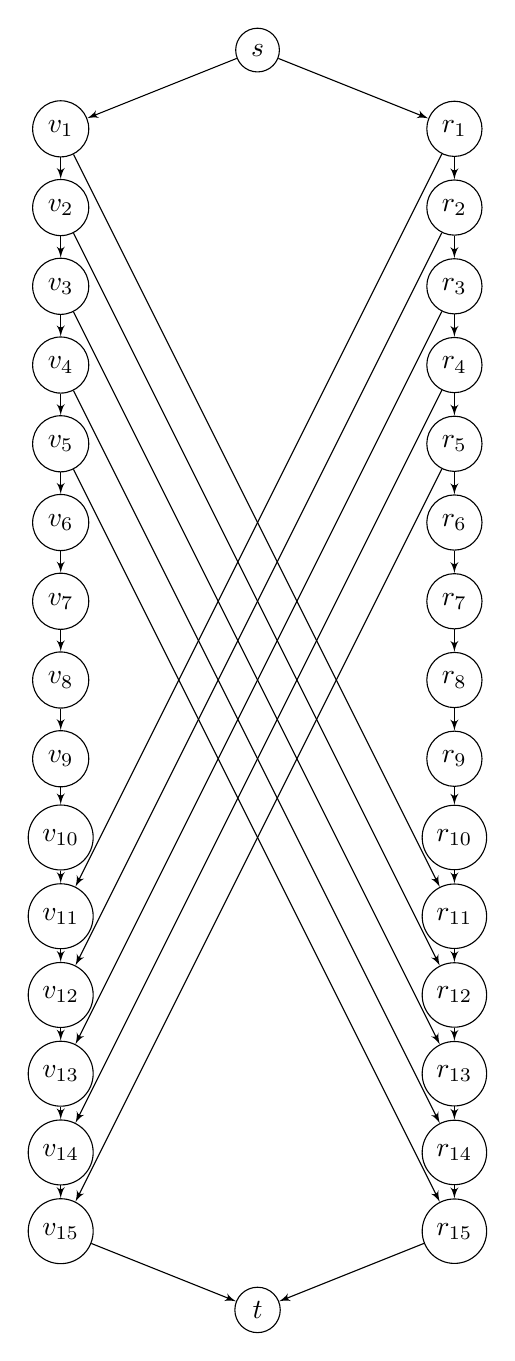
\begin{tikzpicture}

\tikzset{vertex/.style = {shape=circle,draw,minimum size=.1em}}
\tikzset{edge/.style = {->,> = latex'}}
% vertices
\node[vertex] (v1) at  (0,0) {$v_1$};
\node[vertex] (v2) at  (0,-1) {$v_2$};
\node[vertex] (v3) at  (0,-2) {$v_3$};
\node[vertex] (v4) at  (0,-3) {$v_4$};
\node[vertex] (v5) at (0,-4) {$v_5$};
\node[vertex] (v6) at (0,-5) {$v_6$};
\node[vertex] (v7) at  (0,-6) {$v_7$};
\node[vertex] (v8) at  (0,-7) {$v_8$};
\node[vertex] (v9) at  (0,-8) {$v_9$};
\node[vertex] (v10) at  (0,-9) {$v_{10}$};
\node[vertex] (v11) at (0,-10) {$v_{11}$};
\node[vertex] (v12) at (0,-11) {$v_{12}$};
\node[vertex] (v13) at  (0,-12) {$v_{13}$};
\node[vertex] (v14) at  (0,-13) {$v_{14}$};
\node[vertex] (v15) at  (0,-14) {$v_{15}$};

\node[vertex] (r1) at  (5,0) {$r_1$};
\node[vertex] (r2) at  (5,-1) {$r_2$};
\node[vertex] (r3) at  (5,-2) {$r_3$};
\node[vertex] (r4) at  (5,-3) {$r_4$};
\node[vertex] (r5) at (5,-4) {$r_5$};
\node[vertex] (r6) at (5,-5) {$r_6$};
\node[vertex] (r7) at  (5,-6) {$r_7$};
\node[vertex] (r8) at  (5,-7) {$r_8$};
\node[vertex] (r9) at  (5,-8) {$r_9$};
\node[vertex] (r10) at  (5,-9) {$r_{10}$};
\node[vertex] (r11) at (5,-10) {$r_{11}$};
\node[vertex] (r12) at (5,-11) {$r_{12}$};
\node[vertex] (r13) at  (5,-12) {$r_{13}$};
\node[vertex] (r14) at  (5,-13) {$r_{14}$};
\node[vertex] (r15) at  (5,-14) {$r_{15}$};

\node[vertex] (s) at  (2.5, 1) {$s$};
\node[vertex] (t) at  (2.5, -15) {$t$};

%edges
\draw[edge] (s) to (v1);
\draw[edge] (s) to (r1);
\draw[edge] (r15) to (t);
\draw[edge] (v15) to (t);

\draw[edge] (v1) to (r11);
\draw[edge] (v2) to (r12);
\draw[edge] (v3) to (r13);
\draw[edge] (v4) to (r14);
\draw[edge] (v5) to (r15);
\draw[edge] (r1) to (v11);
\draw[edge] (r2) to (v12);
\draw[edge] (r3) to (v13);
\draw[edge] (r4) to (v14);
\draw[edge] (r5) to (v15);

\draw[edge] (v1) to (v2);
\draw[edge] (v2) to (v3);
\draw[edge] (v3) to (v4);
\draw[edge] (v4) to (v5);
\draw[edge] (v5) to (v6);
\draw[edge] (v6) to (v7);
\draw[edge] (v7) to (v8);
\draw[edge] (v8) to (v9);
\draw[edge] (v9) to (v10);
\draw[edge] (v10) to (v11);
\draw[edge] (v11) to (v12);
\draw[edge] (v12) to (v13);
\draw[edge] (v13) to (v14);
\draw[edge] (v14) to (v15);

\draw[edge] (r1) to (r2);
\draw[edge] (r2) to (r3);
\draw[edge] (r3) to (r4);
\draw[edge] (r4) to (r5);
\draw[edge] (r5) to (r6);
\draw[edge] (r6) to (r7);
\draw[edge] (r7) to (r8);
\draw[edge] (r8) to (r9);
\draw[edge] (r9) to (r10);
\draw[edge] (r10) to (r11);
\draw[edge] (r11) to (r12);
\draw[edge] (r12) to (r13);
\draw[edge] (r13) to (r14);
\draw[edge] (r14) to (r15);

\end{tikzpicture}

\newpage
\noindent
This of course, in our problem, will have a LOT more vertices and edges, because who the heck is going to consider switching coffee shops in between the span of 15 minutes. But anyways, as a subproblem, we want to find the maximum weight path, and note along the way when we switch from one coffee shop to the other. \\
\\
To find the longest weight path, we can consider each vertex in order from earliest time to latest. For each time $t$, we will first consider $v_t$ and then $r_t$. This is not for any particular reason, the two are interchangeable. Thus, our vertices will be looked at in our main loop in the following order:\\
Vertices : $\{s, v_1, r_1, v_2, r_2, ..., v_n, r_n, t\}$\\
\\
Now, consider the following:\\
\\
$work[v] = -1$ for all vertices $v$.\\
$prev[v] = null$ for all vertices $v$\\
for every vertex $v$ in cronological order:\\
\indent for every (neighboring vertex of $v$), $u$:\\
\indent \indent if $(work[u] < work[v] + weight[v])$:\\
\indent \indent \indent $work[u] = work[v] + weight[v]$.\\
\indent \indent \indent $prev[u] = v$.\\
\\
To find where Charlie switches coffee shops, simply reccur backwards from $t$ to $s$, and note when the previous of a vertex $v$ is a different coffee shop than $v$. When we look at prev[v], we will get another vertex. For the sake of simplicity, assume we can tell by the name of the vertex (whether it is R or V), that a vertex is location Valve or Ruru. Consider:\\
\\
$switches = \{\}$\\
$location = prev[t]$.\\
while $(prev[location] \neq null)$\{\\
\indent if $prev[location] \neq location$\\
\indent \indent add $prev[location]$ to switches.\\
\indent $location = prev[location]$.\\
\}\\
\\
$switches$ should now contain all the vertices that Charlie is located right before he switches to the other coffee shop.

\newpage
\onecolumn
\noindent
If we didn't want to construct a graph, this can be written as the following, less intuitive, algorithm:\\
\\
$work[t] = -1$ and $prev[u] = null$ for all times at either coffee shop $v_1$ to $v_n$, and $r_1$ to $r_n$.\\
$work[v_1] = 0$
$work[r_1] = 0$
for $t$ (from 1 to $n-1$):\\
\indent if $work[v_{t+1}] < work[v_{t}] + v_t$\\
\indent \indent $work[v_{t+1}] = work[v_{t}] + v_t$\\
\indent \indent $prev[v_{t+1}] = v_{t}$\\
\indent if $v_{t+10}$ is defined\\
\indent \indent if $work[v_{t+10}] < work[v_{t}]$\\
\indent \indent \indent $work[v_{t+10}] = work[v_{t}]$\\
\indent \indent \indent $prev[v_{t+10}] = v_{t}$\\
\indent if $work[r_{t+1}] < work[r_{t}] + r_t$\\
\indent \indent $work[r_{t+1}] = work[r_{t}] + r_t$\\
\indent \indent $prev[r_{t+1}] = r_{t}$\\
\indent if $r_{t+10}$ is defined\\
\indent \indent if $work[r_{t+10}] < work[r_{t}]$\\
\indent \indent \indent $work[r_{t+10}] = work[r_{t}]$\\
\indent \indent \indent $prev[r_{t+10}] = r_{t}$\\


	\begin{claim}
		The above algorithm correctly determines the most efficient locations to study.
	\end{claim}

	\begin{proof}
		As a base case, consider when n = 1. We consider $v_1$, and assign work[$t$] = $v_1$, because all elements in $V$ are non-negative and $t$ was initialized to -1. We then consider $r_1$ and only if the value of $r_1$ is larger than $v_1$ do we replace the value of $work[t]$ with $r_1$. Thus, we have chosen the correct path.

		Suppose the algorithm is correct for some $k \geq 1$. When n= $k+1$, we look at the value of the vertices with time $k$, and only update the value of the vertices adjacent to $k$ if the value of $k$ and the weight of $k$ is greater than the current value. The vertices adjacent to $k$ can either be of work value -1, or some positive integer. If -1, we update the value. If not, we update only if $work[k]$ + $weight[k]$ is greater than the current. Thus, $t$ will be overwritten with whatever coffeeshop has the highest value of $k+1$.
	\end{proof}

	\begin{claim}
		The time complexity is $O(n)$ and the space complexity is $O(2n)$.
	\end{claim}

	\begin{proof}
		Iterating through each vertex yeilds looping $2n$ times. Each vertex has at most two adjacent vertices, giving us $2n(2)$. With each adjacent vertex, we are doing a single comparison and two assignments if the comparison holds true. The algorithm is $O(2n(2)) \implies O(n)$.

		We have two arrays of size $2n+1$ (work and prev) and a list of switching vertices that can be at most $n/10$ in length (when switching every two minutes). Thus, the space complexity is O($2n+1+n/10) \implies O(n)$.
	\end{proof}

	\newpage


\end{document}
